\subsection{Grafo $\overline{K_n \cup Claw_m}$}
La familia consiste en un grafo $K_n$ y un grafo claw o estrella formado por un nodo y m nodos adyacentes, 
unidos de forma disjunta, que es luego complementado.
\begin{figure}[H]
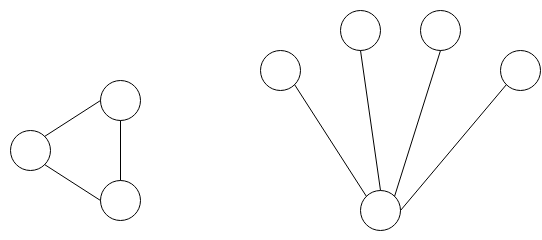
\includegraphics[width=80mm]{K3UC4.png}
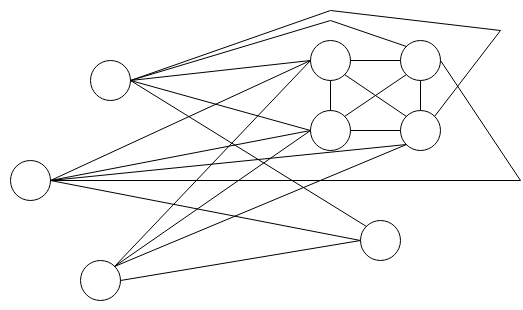
\includegraphics[width=80mm]{K3UC4Complemento.png}
\caption{Ejemplificación: La figura de la izquierda corresponde a $K_3 \cup Claw_4$, 
la figura derecha $\overline{K_3 \cup Claw_4}$}
\label{overflow}
\end{figure}

\subsection{Grafo Completo $K_n$}
Un grafo completo es un grafo simple donde cada par de vértices está conectado por una arista.
Un grafo completo de n vértices tiene n(n-1)/2 aristas.
Es un grafo regular con todos sus vértices de grado n-1.

\begin{figure}[H]
\centering
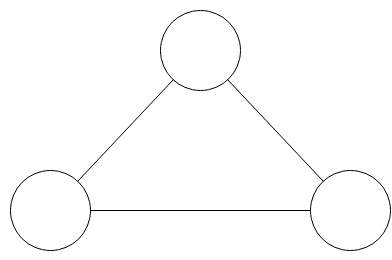
\includegraphics[width=40mm]{K3.png}
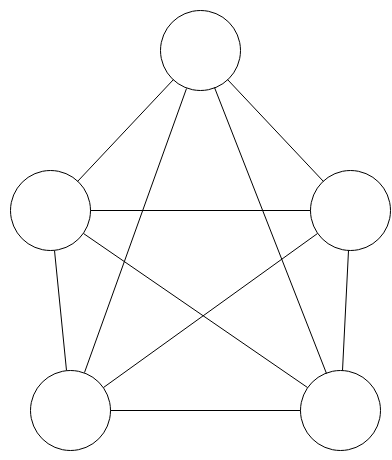
\includegraphics[width=40mm]{K5.png}
\caption{La figura de la izquierda corresponde a un grafo $K_3$ y la figura derecha a un grafo $K_5$.}
\label{overflow}
\end{figure}

\subsection{Grafo Bipartito Completo $K_{n,m}$}
Un grafo bipartito completo es aquel grafo bipartito en el que todos los vértices de la partición $V_1$ están conectados a todos los vértices de la partición $V_2$ y viceversa.

Donde un grafo bipartito es un grafo G=(V,E) cuyos vértices se pueden separar en dos conjuntos disjuntos $V_1$ y $V_2$, es decir, tal que se cumple:
$V_1$ $\cup$ $V_2$ = V
$V_1$ $\cap$ $V_2$ = $\emptyset$
de manera que las aristas sólo pueden conectar vértices de un conjunto con vértices del otro; es decir:
$\forall u_1, u_2 \in V_1, \forall v_1, v_2 \in V_2$ no existe ninguna arista e=($u_1$,$u_2$) ni e=($v_1$,$v_2$).

\begin{figure}[H]
\centering
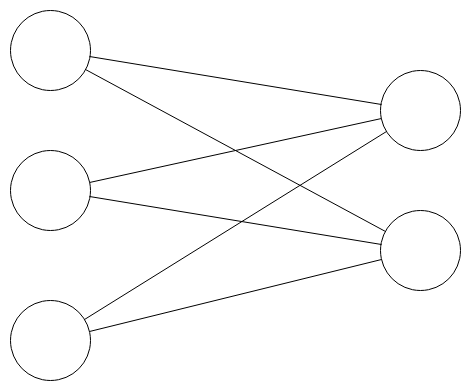
\includegraphics[width=50mm]{K3_2.png}
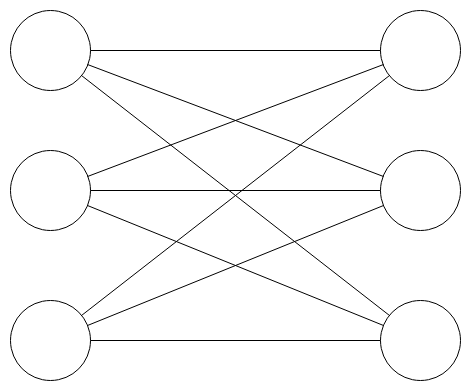
\includegraphics[width=50mm]{K3_3.png}
\caption{La figura de la izquierda corresponde a un grafo bipartito completo $K_{3,2}$ y la figura derecha a un grafo bipartito completo $K_{3,3}$.}
\label{overflow}
\end{figure}


\subsection{Grafo Lattice $L_{m,n}$}
Un grafo Lattice es el producto cartesiano de dos grafos completos $K_m$ y $K_n$.

\begin{figure}[H]
\centering
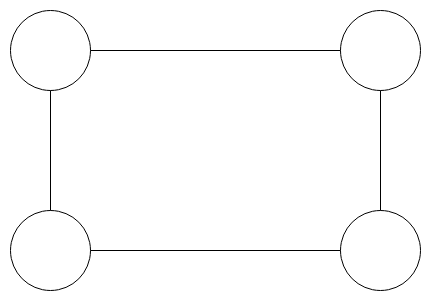
\includegraphics[width=60mm]{L2_2.png}
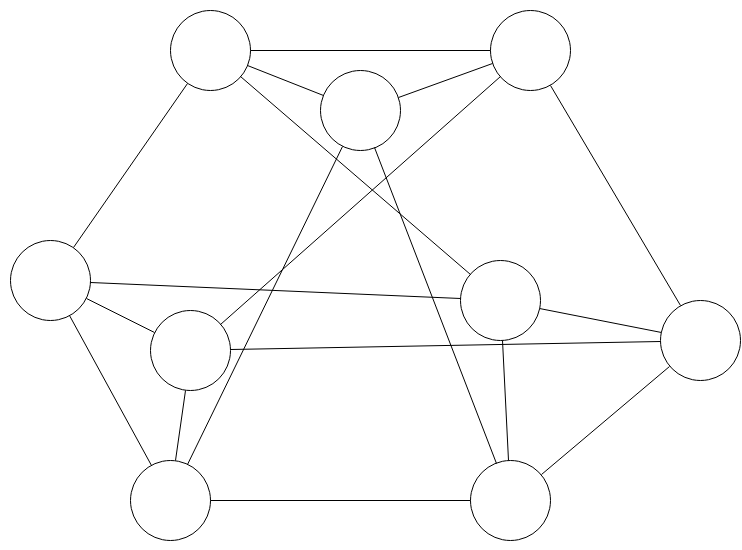
\includegraphics[width=60mm]{L3_3.png}
\caption{La figura de la izquierda corresponde a un grafo Lattice $L_{2,2}$ y la figura derecha a un grafo Lattice $L_{3,2}$.}
\label{overflow}
\end{figure}

\subsection{Grafo Claw}
Un grafo claw es un grafo bipartito completo $K_{1,n}$. Un único vértice que se une con n vértices y entre los n vértices no existen aristas.

\begin{figure}[H]
\centering
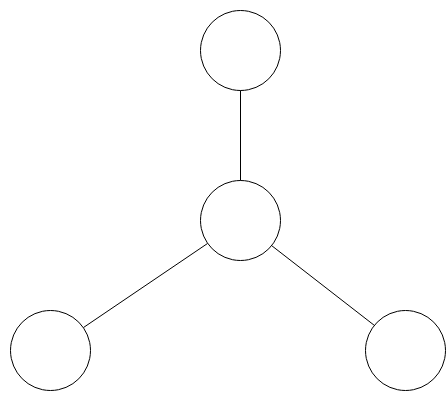
\includegraphics[width=50mm]{K1_3.png}
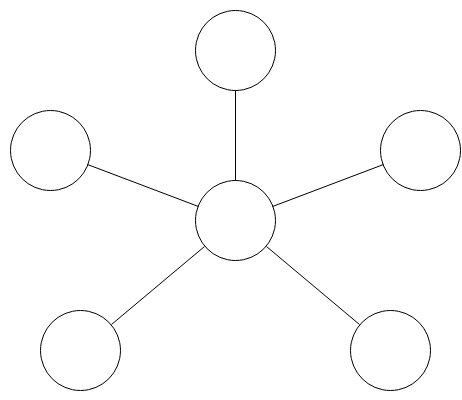
\includegraphics[width=50mm]{K1_5.png}
\caption{La figura de la izquierda corresponde a un grafo claw $K_{1,3}$ y la figura derecha a un grafo claw $K_{1,5}$.}
\label{overflow}
\end{figure}

\subsection{Grafo Path $P_n$}
Un grafo path es un grafo es una sucesión de aristas $e_1e_2$...$e_k$ tal que un extremo de $e_i$ coincide con uno de $e_{i-1}$ y el otro con el de $e_{i+1}$ para i = 2...k-1.

\begin{figure}[H]
\centering
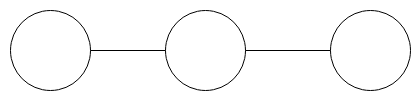
\includegraphics[width=50mm]{P3.png}
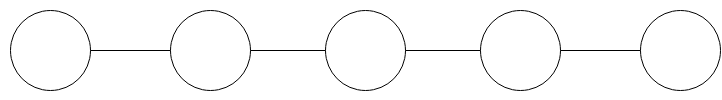
\includegraphics[width=80mm]{P5.png}
\caption{La figura de la izquierda corresponde a un grafo path $P_3$ y la figura derecha a un grafo path $P_5$.}
\label{overflow}
\end{figure}

\subsection{Grafo Fan $F_{m,n}$}
Un grafo fan $F_{m,n}$ se define como la unión de $\overline{K}_m$ y $P_n$.

Donde $\overline{K}_m$ es un grafo con $m$ nodos y 0 aristas y $P_n$ es un grafo path.

\begin{figure}[H]
\centering
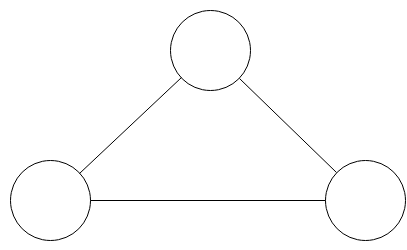
\includegraphics[width=50mm]{F1_2.png}
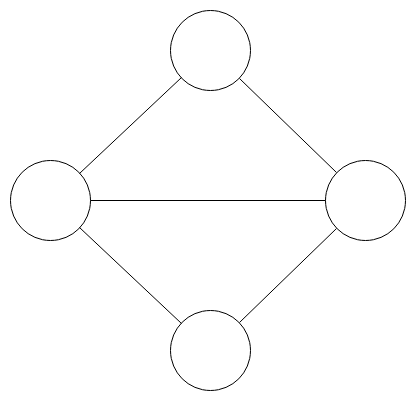
\includegraphics[width=50mm]{F1_3.png}
\caption{La figura de la izquierda corresponde a un grafo fan $F_{1,2}$ y la figura derecha a un grafo fan $F_{1,3}$.}
\label{overflow}
\end{figure}

\subsection{Grafo Cycle $C_n$}
Un grafo cycle $C_n$, es un grafo que se asemeja a un polígono de n lados. Consiste en un camino cerrado en el que no se repite ningún vértice a excepción del primero que aparece dos veces como principio y fin del camino. 

\begin{figure}[H]
\centering
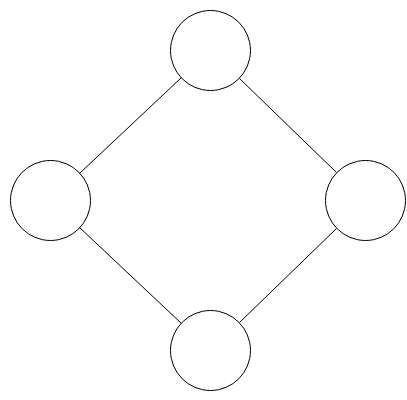
\includegraphics[width=50mm]{C_4.png}
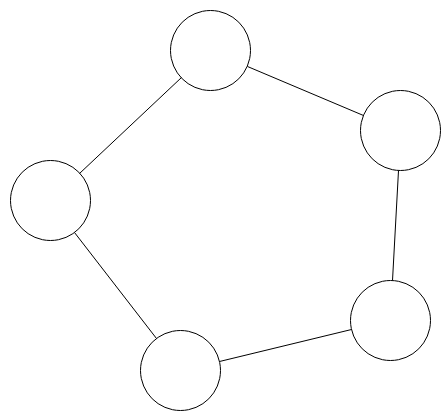
\includegraphics[width=50mm]{C_5.png}
\caption{La figura de la izquierda corresponde a un grafo cycle $C_4$ y la figura derecha a un grafo cycle $C_5$.}
\label{overflow}
\end{figure}

\subsection{Grafo Lollipop }
Un grafo lollipop, es la unión mediante un puente de un grafo completo $K_n$ con un grafo camino path $P_m$. 

\begin{figure}[H]
\centering
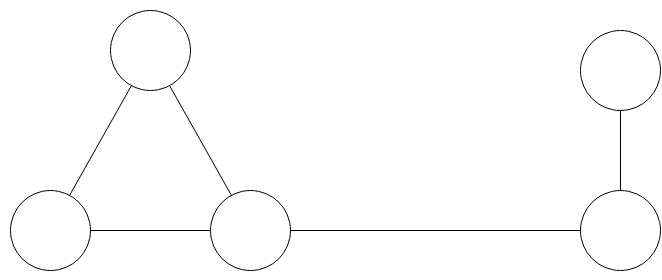
\includegraphics[width=50mm]{lollipop.png}
\caption{La figura corresponde a la unión mediante un puente de un grafo $K_3$ y $P_2$.}
\label{overflow}
\end{figure}


\subsection{Grafo Ninja}
La familia ninja consiste en un grafo claw o estrella donde el nodo central de este será el nodo de mayor grado del grafo, unido por uno de los nodos de su frontera a uno de los nodos de la frontera de un grafo clique de tamaño determinado donde todos sus nodos tendrán el grado máximo posible (grado máximo - 1). Esta familia presenta malos casos para el algoritmo goloso y el local.

\begin{figure}[H]
\centering
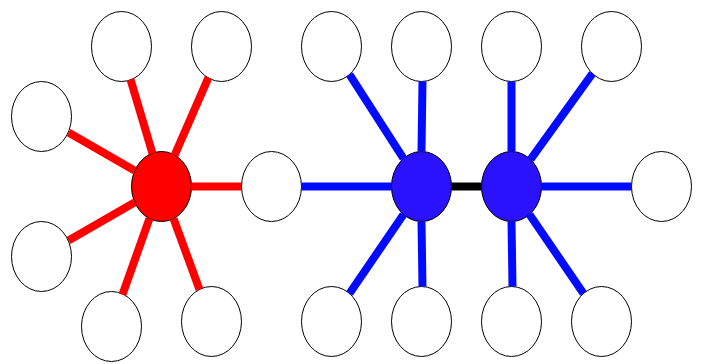
\includegraphics[width=80mm]{ejemploErrorGoloso.png}
\caption{Ejemplificación: Las aristas de color rojo forman parte de la frontera encontrada por los algoritmos, mientras que las aristas de color azul forman la frontera máxima}
\label{overflow}
\end{figure}

Analizando este grafo, puede determinarse que es posible manipular o generar diferentes casos de esta familia para conseguir una respuesta tan mala como se desee.

Incrementando la cantidad de adyacentes del nodo de mayor grado (nodo de color rojo), podemos hacer que el verdadero clique (parte azul) crezca, pudiendo incrementar la diferencia entre la frontera encontrada por el algoritmo y la frontera máxima del grafo provista por una clique.

Tanto el algoritmo goloso, como el algoritmo local (comenzando desde el goloso o desde el nodo de mayor grado) quedarán atascados en el nodo de mayor grado, ya que ningún movimiento que pudieran realizar mejorará la frontera.

Tomando \textbf{d} = nodo de grado máximo y \textbf{c} = tamaño de clique elegido para sección azul, obtenemos que es posible calcular la frontera máxima según el tamaño del clique elejido y del grado máximo que puede encontrarse en el grafo.

La ecuación de la frontera es la siguiente: $f(c) = (d - (c - 1)) * c$.

Buscamos el \textbf{c} máximo para los valores de d. $f'(c) = d - 2 * c + 1$ = 0 $\Leftrightarrow$ $c = (d + 1)/2$.

Es posible corroborar que $c = (d + 1)/2$ es un máximo viendo: $f''((d + 1)/2) = -2 < 0$.

Conociendo \textbf{c}, solo basta con hacer crecer el grado del nodo de mayor grado y conectarlo con un clique de tamaño $(d + 1)/2$ para obtener una diferencia de exactitud en tamaño de frontera de $(d - (c - 1)) * c$ - $d$, que se irá incrementado a medida que d crezca.